\section{Design}
\label{sec:design}

\begin{figure*}[t]
    \centering
    \begin{subfigure}{0.3\linewidth}
        \begin{align*}
            L_1 &= h_1(k) \\
            L_2 &= L_1 + (h_2(k)\mod f^{f + log_2(h_3(k))})
        \end{align*}
        % \caption{}
        % \label{fig:hash_factor}
    \end{subfigure}
    \begin{subfigure}{0.3\linewidth}
        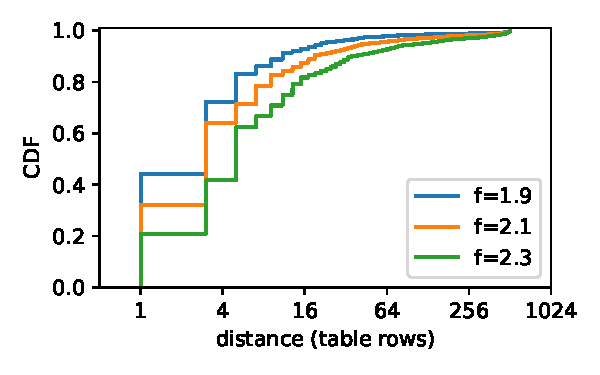
\includegraphics[width=0.99\linewidth]{fig/hash_factor.pdf}
        % \label{fig:hash_factor}
        % \caption{}
    \end{subfigure}
    \begin{subfigure}{0.3\linewidth}
        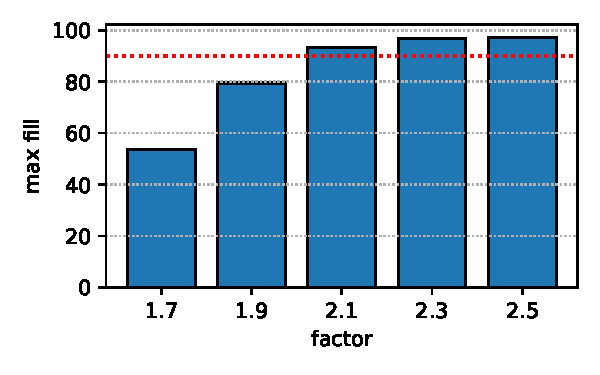
\includegraphics[width=0.99\linewidth]{fig/hash_fill.pdf}
        % \label{fig:hash_fill}
        % \caption{}
    \end{subfigure}.
    \vspace{-1em}
    \caption{
    \textbf{(a)} Dependent hashing for factor $f$.
    \textbf{(b)} CDF of distances between cuckoo locations dependent hashing on different exponential factors.
    \textbf{(c)} Exponential factor relation to max fill in cuckoo hash.
    }
    \label{fig:locality-hashing}

\end{figure*}




\subsection{Locality Hashing}
Both cuckoo~\cite{cuckoo} and hopscotch~\cite{hopscotch}
hashes are optimized for reads. Cuckoo hashing ensures
constant time reads, while hopscotch hashing ensures that a
read is within a bounded range of it's hash index. Both of
these properties have been noticed by the RDMA key-value
store and far-memory communities for their fast
reads~\cite{memc3,cuckoo-improvements,pilaf,farm}.

Our approach aims to combine the bounded reads of cuckoo hashing with
the locality properties of hopscotch hashing.  To do so we make our
two hash functions \textit{dependent}, resulting in a bound on the
distance between cuckoo hash locations.  The first, independent, hash
function selects a uniformly random location, while the dependent hash
selects a second location that is selected uniformly at random from a
(variable-size) region immediately following the first.  To avoid hot
spots, we randomly select the size of the region according to an
exponential distribution with a tuning factor $f$, so that most
locations are close together.
%The second hash function determines the maximum
%distance the second value can have from the first. A third
%hash function determines a random location between the first
%location, and the bound imposed by the second.
Figure~\ref{fig:locality-hashing}(a) shows the formula for our hashing
function process, which implements the probabilistic region-size
selection with a third hash function---akin to the way Bitcoin
computes its difficulty.
\textbf{Why not make the second hash function a true expoential?}

A strawman implementation of locality based hashing would
use the first hash function to find a location, and the
second to find a random location within a fixed bound. This
approach quickly leads to failed insertions. Due to the
birthday paradox the probability of a collision is high, and
on large tables the probability that one region of the hash
table will become full, and have not viable path to an open
slot is high. ~\sg{Perhaps this justifies a figure, please
advise.}.

We use a dynamic exponential bound rather than a static one.
The dynamic bound is set by raising a constant factor $f$ by
an exponent determined by a third hash function. Using the
third hash on the key we count the number of suffix zeros
and raise the constant factor by itself plus the zero count.
This distribution generates exponential distances between
hash locations at exponentially less frequency and is
tunable with the single parameter $f$.
%%
In the common case the bound is small. Exponentially few key
are spaced far apart and act as~\textit{waypoints} to other
regions of the table when constructing cuckoo paths. This
method, paired with bucket associativity enables high fill
rates while keeping the region of the table any given key
can inhabit small.

There is a tradeoff between locality and fill factor.
Figure~\ref{fig:locality-hashing}(b) illustrates how
increasing the exponential factor shifts the distribution of
distances between cuckoo hash locations.
Figure~\ref{fig:locality-hashing}(c) shows how these same
factors effect the max fill rate of the table before an item
cannot be inserted. As will be shown in the following
sections read, and insert performance improve with better
locality. Therefore fill factor and performance can be
traded off directly by changing the exponential factor. In
our evaluation we found an exponential factor of 2.3 to give
the best results in terms of end to end performance and
bandwidth consumption.


\subsection{Locking}

\begin{figure*}[t]
    \centering
    \begin{subfigure}{0.3\linewidth}
        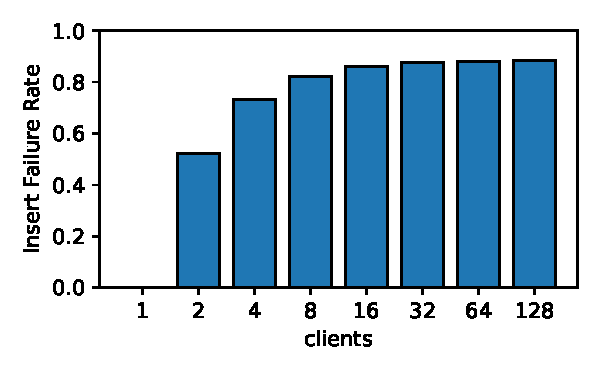
\includegraphics[width=0.99\linewidth]{fig/optimistic_failures.pdf}
        % \label{fig:optimistic_failures}
        % \caption{}
    \end{subfigure}
    \begin{subfigure}{0.3\linewidth}
        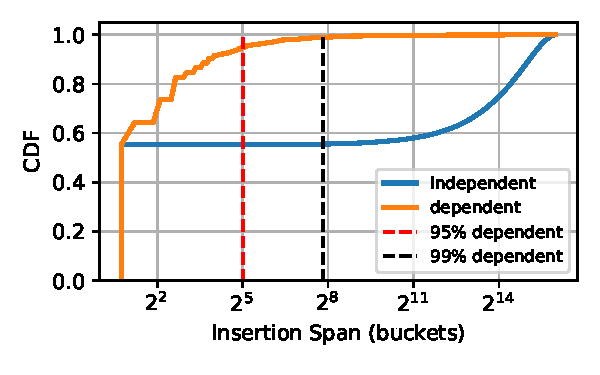
\includegraphics[width=0.99\linewidth]{fig/insertion_span.pdf}
        \label{fig:insertion_span}
        % \caption{}
    \end{subfigure}.
    \begin{subfigure}{0.3\linewidth}
        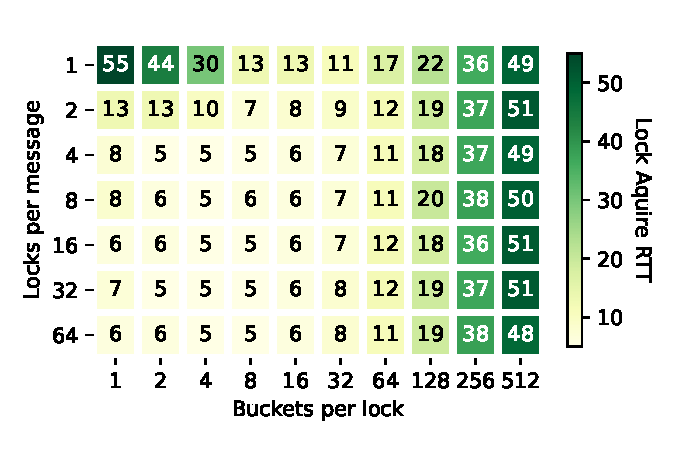
\includegraphics[width=0.99\linewidth]{fig/buckets_per_lock_vs_locks_per_message.pdf}
        \label{fig:tbd}
        % \caption{}
    \end{subfigure}.
    \vspace{-1em}
    \caption{
    \textbf{(a)} Failure rate of optimistic cuckoo insertions.
    \textbf{(b)} CDF of cuckoo spans for dependent and independent hashing. A cuckoo span is the distance between the smallest and largest index in a cuckoo path.
    \textbf{(c)} Round trips (99th percentile) required per insert while filling a table to 100\% while varying the lock per message, and buckets per lock. \todo{subtract one from each current values include unlocks}
    }
    \label{fig:cuckoo-problems}

\end{figure*}



Traditional wisdom would suggest that because cuckoo hashing
can have long insertion paths it is a poor candidate for
remote memory. Both opportunistic, and lock based approaches
have significant drawbacks.
%%
As an example consider an opportunistic approach in which
many clients are inserting concurrently to a table. Clients
making inserts first make reads of the table to locally
calculate a cuckoo path for their insertion. After the reads
complete the client constructs a cuckoo path and starting
from the open slot issues dependent CAS requests migrating
the open slot backwards to the insertion bucket.
%%
Figure~\ref{fig:cuckoo-problems}(a) shows the failure rate
of this insertion scheme as a factor of clients running
inserts on a table with 500K entries with a bucket
associativity 8. Cuckoo paths calculated from client caches
quickly become invalid as the number of clients grows.
%%
Alternatively deadlock free lock acquisition requires more
round trips and has larger critical sections. Each lock must
be acquired in order with a dependent CAS request which
incurs an additional round trip per lock. Using course
grained locks reduces the number of acquisitions but
throttles throughput as concurrent insertions are more
likely to contend shared locks.

Locality hashing increases the probability that an insertion
path is within a small region of the hash table which in
turn increases the probability that fine grained locks will
be near one another. 
%%
Figure~\ref{fig:cuckoo-problems}(b) shows the insert span in
buckets using both dependent and independent hashing on a
table with 500K entries and an associativity of 8. A span is
calculated as the distance between the lowest index and the
highest index in a cuckoo path. Past 50\% independent
hashing spans a random range in the table (whenever a
displacement occurs on insert). With dependent locality
based hashing 95\% of inserts span less than 32 buckets, and
99\% less than 256.
%%
RDMA masked CAS operations allow a client to set a 64 bit
mask along with the new, and old values of the cas
operation. So locks can be acquired with minimal knowledge
of the remote lock table. This enables the client to
atomically set up to 64 contiguous locks independently which
dramatically reduces the round trips required to aquire
locks.

Lock granularity effects performance under contention. Using
values from Figure~\ref{fig:cuckoo-problems}(b) if locks are
per bucket 96\% of lock acquisitions can be completed with a
single RTT masked cas. If locks span 4 buckets 99\% of
requests can be completed in a single round trip.
%%
Figure~\ref{fig:ycsb_fill_latency}(c) shows the tradeoff between lock
granularity and the number of locks which can be set in a
single message with locality hashing turned on. The values
reported are the 99th percentile number of round trips
required to acquire locks up to a 90\% fill factor on a
table with 4096 entries and 8 entries per bucket, and 8
concurrent clients. The biggest factor in round trip times
is the number of locks per bucket. On the far right side of
the heatmap (512) only a single global lock exists. Further
the benefit in terms of locks per message falls off quickly
after two. RDMA-masked CAS are beneficial as they allow for
fine-grained locking, but setting 3 or more locks per
message has little effect up to 90\% fill rate. Reducing
atomic operations in turn reduces the effect of the RDMA
atomic bottleneck.  \textbf{Hard to see 3; the figure only shows 2 or 4.}

Our lock table is small in comparison to the true hash
table. At its most fine-grained each lock corresponds to
one bucket (8 entries). Each lock is 1 bit, a lock table for
a 100 million entry hash table is ~160KB, with a lock
granularity of 4 buckets this drops to 40KB. This tight
layout enables us to use device-mapped memory to hold our
lock table~\cite{design-guidelines,sherman}.
%We make use of
Device-mapped memory on recent RDMA NIC's (ConnectX-5+) avoids an
expensive PCIe round trip, reducing lock acquisition latency.
This enables up
to 3$\times$ better throughput on contested locks (see
Figure~\ref{fig:rdma-benchmarks}(c)), and reduces latency
for locking.

\subsection{Table Design}

We design our table with flexibility in mind. Our goal is to
support inlining fixed sized keys and values in the index,
while simultaneously supporting variable sized values.
Unlike one-sided hash functions which have their index
entries limited to a CAS width~\cite{race}, rcuckoo supports
variable sized entries because updates are guarded by client
held locks rather that RDMA CAS operations. Inlining entries
has the benefit that reads require a single round trip,
their halfing their latency. Further keys can be stored
directly in the index, not just their
digests~\cite{pilaf,race}, this too removes the need to read
extent data to verify that an index entry matches it's true
key. Figure~\ref{fig:table-diagram} illustrates our table
design.  Each entry includes an extent bit to indicate if
the entry is inlined or stored in an extent.



\begin{figure}[t]
    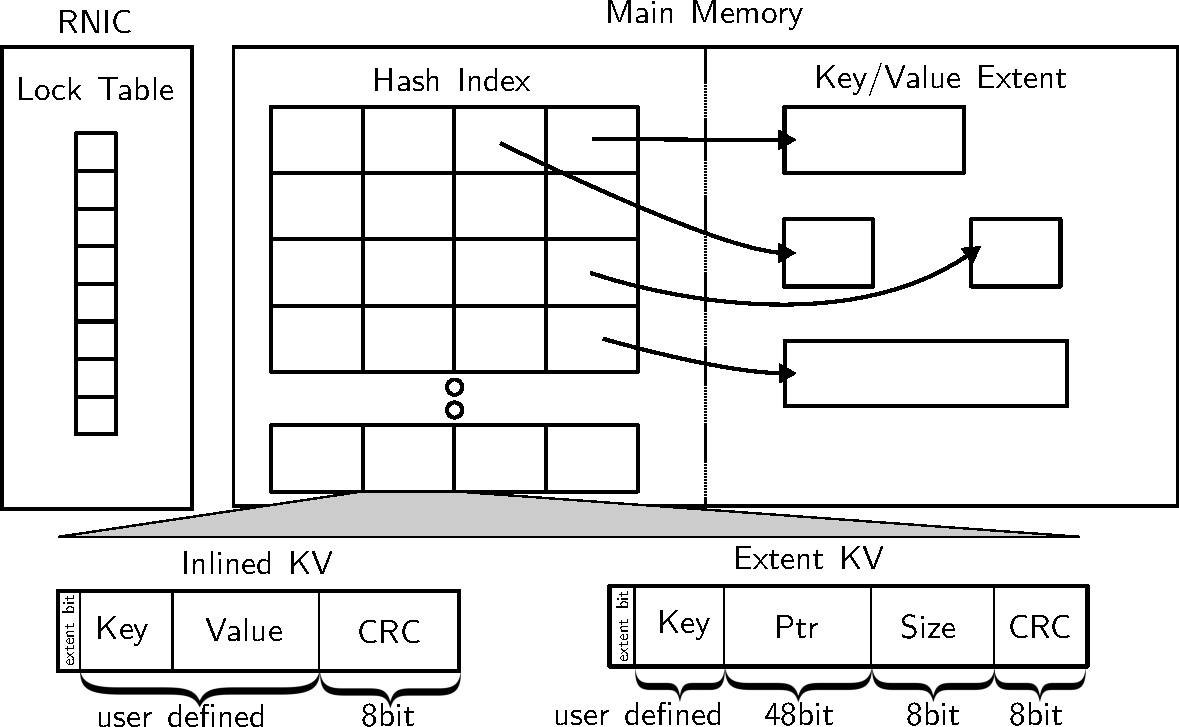
\includegraphics[width=0.99\linewidth]{fig/table-diagram.pdf}
    \caption{Rcuckoo's table design}
    \label{fig:table-diagram}
\end{figure}


\subsection{Protocol}

\begin{figure}[t]
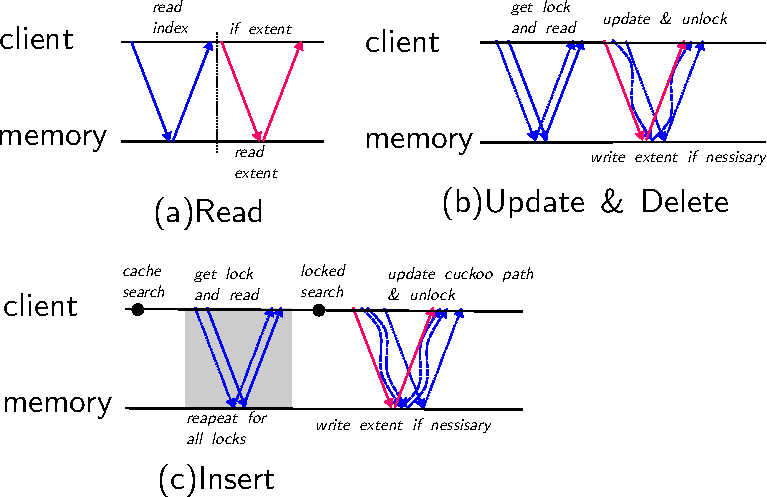
\includegraphics[width=0.99\linewidth]{fig/message_diagram.pdf}

\caption{Rcuckoo's protocol for reads, inserts, deletes and
updates. Blue lines are index accesses, and red lines are
extent accesses. Solid lines are reads, dotted lines are
CAS, and curved dashed lines are writes.}

\label{fig:message_diagram}
\end{figure}

In this section we describe our protocol for reading,
inserting, and performing updates and deletes to an rcuckoo
hash table. Figure~\ref{fig:message_diagram} visualizes our
protocol.

\subsubsection{Reading} All reads are performed locklessly.
If keys and values are inlined clients complete reads in a
single round trip, otherwise a second round trip is required
to resolve a pointer and read the extent. 
%%
~\footnote{This design requires exactly one pointer
resolution in expectation that future RDMA NICs may provide
pointer resolution reads as a primitive~\cite{prism}}
%%
The index is modified concurrently by writes, clients must
therefore validate their reads by computing a CRC post
read~\cite{pilaf,cell}.
%%
In the base case clients compute both hash locations for a
key and issue two bucket sized RDMA read requests to the
index. As an optimization clients can perform reads using a
single packet. We define a read threshold of 512 bytes for
our clients, if two hash locations are within 512 bytes we
issue a single large read.  Approximately 60\% of keys for
64-bit entries with a bucket size of 8 (see
Figure~\ref{fig:locality-hashing}(b)) fall into this
category. This has the advantage of updating the client
cache for future operations.
%, and reduces the header
%processing required by the NIC.
To reduce bandwidth the size
of the threshold can be tuned down, or turned off with no
harm to correctness.

\subsubsection{Locking and unlocking}

Update, delete and insertion operations all require locks to
modify the index. Locks are acquired in incremental order
from smallest to largest to avoid deadlocks. First the list
of locks required for the operation is calculated. For
updates and deletes this requires a single lock, for insert
many locks may be required. Once the client has calculated
which buckets it needs to lock it computes a list of RDMA
masked CAS requests. If the locks required are within 64
locks of one another they are batched together into a single
masked CAS request. After the list is computed the client
issues lock requests one CAS at a time. If a request
fails that request is retried until the lock is acquired.

Clients need their caches synchronized with remote memory
prior to modifying it with writes. We batch reads with lock
requests to synchronize client caches. RDMA in-order
delivery ensures that reads issued after a lock request will
be up to date, as no other client can concurrently modify
the locked index.  A spanning read is issued for each lock
request. The read covers each bucket the client locks.  For example, if a
masked CAS has three locks, reads are calculated for each
bucket being locked. If the locks cover a range less than
the read threshold a single read is issued which spans all
buckets between the locks.  Spanning reads are issued concurrently with
lock requests.
%Subsequent lock requests are issued prior to
%blocking on reads.

After locks are acquired the client can execute its critical
section. Unlock requests are the inverse masked CAS operations of the
lock requests. Clients issue their critical sections as a sequence of
(asynchronous) writes followed immediately by unlock operations. RDMA
in-order delivery ensures that the unlock operations are performed
after the writes.

\subsubsection{Updates and Deletes}

Updates and deletes are performed in a similar fashion.
First the client aquire locks for the key it will update or
delete. If the key exists the client updates its value with
a write and then releases the locks. For updates the client
updates the value and the CRC of the index, for deletes the
index is simply set to NULL. If extents are being used
updates asynchronously write their extent data during lock
acquisition. Both updates and deletes for extents remove the
old extent data lazily. Regardless of if extents are turned
on updates and deletes are performed in two round trips.

\subsubsection{Insert}

Unlike updates and deletes, inserts may require modifying locations spread across remote memory and
require many locks. Determining which locks are required is
hard as clients may have stale caches. We use a two-phase
search strategy to find insertion paths. First the client
constructs a potential cuckoo path using its cached index. The client
then attempts to acquire the locks necessary for its cuckoo path. Thanks to the spanning reads, once a client succeeds in acquring the necessary locks its
cache has been fully synchronized with the relevant portions of remote memory. A second
search is then performed using only the buckets the client
succeeded in locking---which may be the same if the client's cache was completely up to date. If this search is successful the client
calculates the updates to the cuckoo path batches them as a
series of writes and issues them along with it's unlock
requests.

If the first search fails the client performs a read and
tries again. If this fails the table must be resized. The
second search may fail because the clients cache was stale
and the list of locked buckets was insufficient to perform
the insert. In this case the client releases the locks and
performs the insertion from the start again by performing an
unrestricted search on its local cache. In the common case
insertions take two round trips: We find that when the table is less
than 50\% full the probability that a cuckoo path has
length greater than one is low. If extents are
used the client batches the extent write during its locking
phase.

\textbf{Key Duplication:} Unlike RACE our algorithm can
prevent duplicate keys easily on insert~\cite{race}. RACE
requires three round trips for inserts, the third re-reads
the index to ensure no duplicates were inserted
concurrently.  Alternatively Cuckoo hashing inserts to
exactly one bucket, which is read during the lock
acquisition phase. If a duplicate key is found the client
can abort. If the bucket is full, a duplicate key may exist
in itts alternative bucket. Our clients issue a read to the
inserted keys alternative bucket during lock acquisition. If
the lock returns successfully and no duplicate exists in
either bucket then no duplicates exist as the successful
lock ensures that no other client is currently moving the
key to another location as part of a concurrent insert.


\subsubsection{A* Search} 

Locality based hashing provides us opportunities for better
search than traditional cuckoo hashing. Cuckoo hashing
insert traditionally uses random replacement~\cite{cuckoo}.
Random replacement requires little computation, however at
high fill rates it leads to long cuckoo paths which require
many locks, and reduce concurrent throughput. BFS search
finds the shortest path and has been demonstrated to
increase system throughput with fine-grained
locking~\cite{cuckoo-improvements}.  BFS is
computationally intensive. Locality based hashing enables us
to leverage more efficient search strategies. Because
locality hashing increases the probability that a cuckoo
hashing location is close we can use an informed search
algorithm to find open slots close to bucket a key hashes
to. 
%%
In the case of BFS the target bucket is unknown, therefore
all paths must be explored. We use A* search, an algorithm
which takes a goal location, and a distance heuristic as
input. A* is known to find shortest paths in much better
average-case times than BFS~\cite{}. A* requires two additional
inputs, a distance heuristic and a goal location.

\textbf{Goal location}: Locality hashing increases the
probability that an open slot near the insertion target
location can terminate a cuckoo path. Our algorithm collects
open slots near the original hash location as candidate goal
locations. By default we set the number of candidate goal
locations to 5. Goal locations are collected by starting at
the $h_1(k)$ location and iterating through the hash
table both forward and backwards through the table one index
at a time. Buckets with open slots are added to the
candidate list until the limit is reached. 

% \todo{I could
% improve this search time by tracking the list of open
% buckets and using binary search on them.}.

\textbf{Search Heuristic}: A* requires a heuristic for
distance which is a strict underestimate of the true
distance to a goal. A typical heuristic for search is the
euclidean distance between two points. A * guarantees that
if the search heuristic is a strict underestimate of the
true distance to the goal then the path found will be the
shortest path. In our case we use the distance between a
goal state and a current state is unknown as the distance
between any two buckets is the result of our locality
hashing function which has no upper bound. However we can
estimate the distance between two buckets by using the mean
distance of our locality hash function. This approach does
not guarantee that we find the shortest path, however it
does find short paths in the common case, and results in
very short search times.